\subsection{Catálogo Spotify e qualidade dos campos}
O arquivo público disponibilizado no Kaggle por \texttt{amitanshjoshi} sob o nome \textit{Spotify\_1Million\_Tracks} contém 1.159.764 linhas, com identificadores Spotify distintos, e 20 campos \cite{spotifydataset}. Essa é a população finita acessível. A fonte não documenta um desenho de seleção a partir da plataforma inteira. Cada linha é uma faixa, de modo que versões ou gravações de uma composição podem ter IDs diferentes. Há 64.157 créditos de artista distintos como cadeias de caracteres, 882.360 títulos distintos, 15 créditos ausentes e um título ausente. Os campos de identificação não servem como preditores. A Tabela~\ref{tab:dicionario} apresenta o dicionário.

\begingroup\footnotesize\singlespacing
\begin{longtable}{@{}P{.26\linewidth}P{.20\linewidth}P{.48\linewidth}@{}}
\caption{Dicionário dos campos do arquivo Spotify.}\label{tab:dicionario}\\
\toprule Campo & Tipo ou unidade & Definição operacional \\\midrule\endfirsthead
\toprule Campo & Tipo ou unidade & Definição operacional \\\midrule\endhead
\bottomrule\endfoot
\bottomrule\endlastfoot
Sem nome & Índice & Índice exportado no CSV. \\
\texttt{track\_id} & Texto & Identificador da faixa Spotify. \\
\texttt{track\_name} & Texto & Título informado. \\
\texttt{artist\_name} & Texto & Crédito de artista informado. \\
\texttt{popularity} & Inteiro 0--100 & Escore observado de popularidade. \\
\texttt{year} & Ano inteiro & Ano informado na fonte. \\
\texttt{genre} & Categoria & Rótulo de gênero fornecido. \\
\texttt{danceability} & Escore 0--1 & Adequação estimada à dança. \\
\texttt{energy} & Escore 0--1 & Intensidade e atividade percebidas. \\
\texttt{key} & Classe 0--11 & Classe de altura musical, com $-1$ se não identificada. \\
\texttt{loudness} & Decibéis (dB) & Intensidade sonora média informada. \\
\texttt{mode} & Categoria 0/1 & Modo menor ou maior. \\
\texttt{speechiness} & Escore 0--1 & Presença estimada de fala. \\
\texttt{acousticness} & Escore 0--1 & Grau estimado de caráter acústico. \\
\texttt{instrumentalness} & Escore 0--1 & Estimativa de ausência de voz. \\
\texttt{liveness} & Escore 0--1 & Indícios de execução ao vivo. \\
\texttt{valence} & Escore 0--1 & Positividade musical estimada. \\
\texttt{tempo} & BPM & Andamento global estimado. \\
\texttt{duration\_ms} & Milissegundos & Duração da faixa. \\
\texttt{time\_signature} & Categoria & Assinatura de tempo estimada. \\
\end{longtable}
\fonte{Arquivo Spotify\_1Million\_Tracks \cite{spotifydataset} e documentação do Spotify \cite{spotifyaudio,spotifydocs}.}
\endgroup



A popularidade é um escore de zero a cem. A documentação da plataforma associa a medida ao volume e à recência de reproduções \cite{spotifydocs}. A data de medição do escore no arquivo e a versão exata do CSV não foram confirmadas. O ano registrado é usado como metadado fornecido, pois a fonte não permite assegurar que seja o primeiro lançamento da composição. Os atributos acústicos também são fornecidos no arquivo e não foram extraídos novamente do áudio \cite{spotifyaudio}.

\subsection{Distribuições marginais e período}
A popularidade tem média de 18,38, mediana de 15 e percentil 95 de 49. Há 158.391 faixas com escore zero (13,66\%) e 499 com escore entre 80 e 100 (0,043\%). A transformação $\log(1+s)$, para escore $s$, preserva os zeros. Na Figura~\ref{fig:poplog}, ela inverte o sentido da assimetria de $0,810$ para $-0,795$, com pouca mudança em magnitude. O modelo final utiliza os limites na escala original.

\figura[.24\textheight]{02_popularidade_original_log1p}{Distribuição da popularidade nas escalas original e logarítmica.}{fig:poplog}{A escala logarítmica usa $\log(1+s)$.}

O ano informado concentra 443.801 faixas em 2000--2009, 514.990 em 2010--2019 e 200.973 em 2020--2023 (Figura~\ref{fig:anos}). As popularidades médias nesses três grupos são 12,66, 19,99 e 26,89, respectivamente. Essa associação pode refletir a composição da fonte e a relação entre recência e escore. A presença de uma observação por faixa impede acompanhar a evolução individual ao longo do tempo.

\figura[.24\textheight]{04_anos}{Número de faixas por ano informado no catálogo.}{fig:anos}{}

A Tabela~\ref{tab:numericos} resume os atributos numéricos. A instrumentalidade tem mediana de 0,00176 e terceiro quartil de 0,614, ilustrando a grande diferença entre partes da distribuição. As distribuições de presença de fala e de indício de execução ao vivo têm caudas à direita. Dançabilidade se concentra em valores intermediários e energia tem maior presença em escores altos. A duração mediana é 225,74 segundos, com 448,00 segundos no percentil 95 e máximo de aproximadamente 100 minutos. O histograma de amplitude completa torna essa cauda visível. Os quantis caracterizam a região típica com maior resolução.

\begin{table}[H]\centering\footnotesize
\caption{Resumo das variáveis numéricas no catálogo.}\label{tab:numericos}
\setlength{\tabcolsep}{4.0pt}
\begin{tabular}{@{}lrrrrrr@{}}\toprule
Variável & Média & DP & P25 & Mediana & P75 & P95 \\\midrule
Popularidade & 18,38 & 15,89 & 5,00 & 15,00 & 29,00 & 49,00 \\
Ano informado & 2011,96 & 6,80 & 2006,00 & 2012,00 & 2018,00 & 2022,00 \\
Dançabilidade & 0,5374 & 0,1845 & 0,4130 & 0,5500 & 0,6770 & 0,8110 \\
Energia & 0,6397 & 0,2705 & 0,4540 & 0,6940 & 0,8730 & 0,9760 \\
Intensidade sonora (dB) & -8,98 & 5,68 & -10,83 & -7,45 & -5,28 & -3,15 \\
Presença de fala & 0,0928 & 0,1268 & 0,0371 & 0,0507 & 0,0890 & 0,2980 \\
Caráter acústico & 0,3215 & 0,3550 & 0,0064 & 0,1470 & 0,6400 & 0,9760 \\
Instrumentalidade & 0,2523 & 0,3651 & 0,0000 & 0,0018 & 0,6140 & 0,9230 \\
Vivacidade & 0,2230 & 0,2011 & 0,0979 & 0,1340 & 0,2920 & 0,7080 \\
Valência & 0,4556 & 0,2685 & 0,2260 & 0,4380 & 0,6740 & 0,9100 \\
Andamento (BPM) & 121,38 & 29,78 & 98,80 & 121,93 & 139,90 & 174,88 \\
Duração (s) & 249,56 & 149,43 & 181,09 & 225,74 & 286,91 & 448,00 \\
\bottomrule
\end{tabular}\nota{$N=1.159.764$ por variável. O DP usa divisor $N$. Andamento inclui zeros.}
\end{table}


Há 1.199 faixas com andamento zero, das quais 650 pertencem ao gênero \textit{sleep}. Os registros foram preservados no catálogo e nos momentos do dimensionamento. A descrição gráfica de andamento e as análises de correlação e PCA usam a regra de andamento positivo. O tratamento separa explicitamente esses denominadores. Os campos numéricos de áudio e duração aparecem na Figura~\ref{fig:distacustica}.

As categorias musicais também exibem concentração. O modo maior corresponde a 63,47\% das faixas. A assinatura de tempo codificada como 4 responde por 87,14\%. Na tonalidade, as classes mais frequentes são 7 (12,04\%) e 0 (11,22\%). Essas variáveis são tratadas como categorias na modelagem. A Figura~\ref{fig:categoriasmusicais} apresenta a distribuição completa de seus níveis.

\figura[.54\textheight]{01_distribuicoes_metadados}{Distribuições dos dez atributos acústicos e de duração.}{fig:distacustica}{Cada painel informa o número de valores válidos.}
\figura[.23\textheight]{05_categorias_musicais}{Tonalidade, modo e assinatura de tempo no catálogo.}{fig:categoriasmusicais}{}

\subsection{Gênero e perfis acústicos}
O catálogo tem 82 rótulos de gênero. \textit{Black-metal} é o mais frequente, com 21.852 faixas (1,88\%). \textit{Songwriter} reúne 589 (0,05\%). Os rótulos são mantidos como no arquivo e incluem estilos, usos ou contextos de escuta. As frequências caracterizam a fonte, que não mede participações de mercado. A Figura~\ref{fig:generos} mostra os vinte rótulos mais frequentes.

\figura[.35\textheight]{03_generos}{Vinte rótulos de gênero mais frequentes no catálogo.}{fig:generos}{A tabela de frequências que acompanha o projeto inclui os 82 rótulos.}

Para uma variável $z$ com média $\bar z$, a fração de variação associada às diferenças entre $G$ médias de grupos é
\begin{equation}
\eta^2=\frac{\sum_{g=1}^G N_g(\bar z_g-\bar z)^2}{\sum_i(z_i-\bar z)^2},
\end{equation}
com $N_g$ igual ao número de valores válidos do grupo $g$. Assim, 51,76\% da soma de quadrados de caráter acústico corresponde a diferenças entre gêneros. Para presença de fala, intensidade sonora, energia, dançabilidade, popularidade, instrumentalidade e andamento válido, as frações são 49,96\%, 48,39\%, 45,99\%, 41,86\%, 41,27\%, 40,10\% e 8,50\%, respectivamente. A energia média varia de 0,222 em \textit{classical} a 0,933 em \textit{death-metal}. Isso sustenta a estratificação do sorteio por gênero e indica a necessidade de conferir atributos que variam substancialmente dentro dos gêneros.

As Figuras~\ref{fig:perfis_a} e~\ref{fig:perfis_b} mostram os 82 perfis. Cada célula é a diferença entre a média do gênero e a média do catálogo, expressa em desvios-padrão do campo. O contraste entre energia, intensidade sonora e caráter acústico aparece em vários rótulos. Na Figura~\ref{fig:boxgenres}, os intervalos entre quantis evidenciam a heterogeneidade dentro dos próprios gêneros.

\begin{figure}[!htbp]
\centering
\begin{minipage}[t]{.485\linewidth}
\centering
\caption{Perfis padronizados dos gêneros 1 a 41 em ordem alfabética.}
\label{fig:perfis_a}
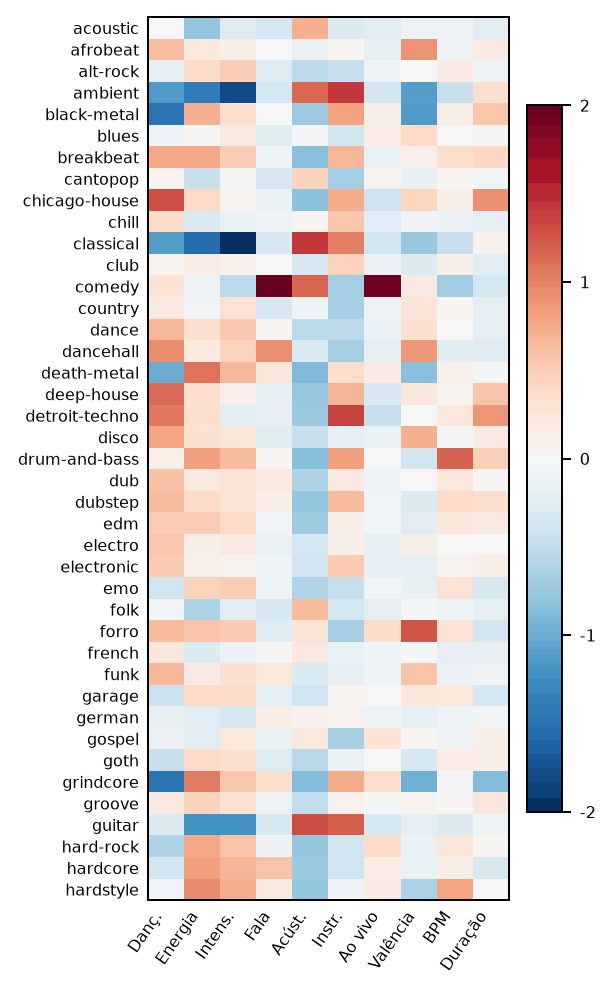
\includegraphics[width=\linewidth]{images/perfil_generos_1.png}
\end{minipage}\hfill%
\begin{minipage}[t]{.485\linewidth}
\centering
\caption{Perfis padronizados dos gêneros 42 a 82 em ordem alfabética.}
\label{fig:perfis_b}
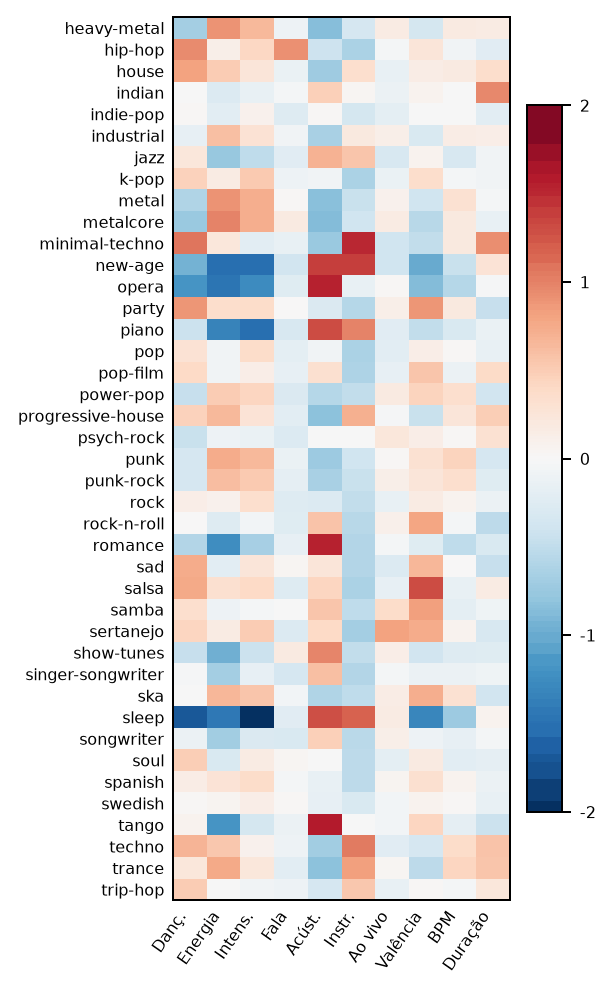
\includegraphics[width=\linewidth]{images/perfil_generos_2.png}
\end{minipage}
\nota{Escala comum em desvios-padrão. Danç. = dançabilidade, Intens. = intensidade
sonora, Acúst. = caráter acústico e Instr. = instrumentalidade.}
\end{figure}

Entre os exemplos do segundo painel, \textit{sleep} tem andamento válido médio de aproximadamente 100 BPM. Em \textit{drum-and-bass}, no primeiro painel, a média é de 157 BPM. Já a instrumentalidade média é de 0,0025 em \textit{sertanejo} e 0,767 em \textit{ambient}. O padrão por gênero é útil para o desenho amostral e para interpretar a perda de cobertura quando um gênero tem poucas faixas vinculadas.

\figura[.49\textheight]{09_distribuicoes_por_genero}{Atributos selecionados nos dez gêneros mais frequentes.}{fig:boxgenres}{Hastes nos percentis 5 e 95, caixas entre os quartis e traço na mediana.}

No agrupamento por período, as diferenças entre médias representam menos de 1\% da variação de cada atributo acústico ou de duração. Para a popularidade, a fração é 10,39\%. Na Figura~\ref{fig:perfilperiodos}, a escala padronizada é a mesma usada na comparação entre gêneros. Os contrastes menores entre períodos são coerentes com os valores de $\eta^2$.

\figura[.25\textheight]{08_perfis_periodos}{Perfis acústicos médios por período, em escala padronizada.}{fig:perfilperiodos}{Diferenças medidas em desvios-padrão em relação ao catálogo.}

\subsection{Associações entre atributos e componentes principais}
O conjunto de casos completos para as análises bivariadas reúne 1.158.565 faixas. A Figura~\ref{fig:corr} apresenta as correlações de Pearson e Spearman nas mesmas observações. Por Pearson, energia tem correlação de 0,781 com intensidade sonora e de $-0,754$ com caráter acústico. Dançabilidade e valência têm correlação de 0,518. As direções principais se mantêm nas correlações de postos. As densidades da Figura~\ref{fig:densidades} mostram concentrações e variações conjuntas que um único coeficiente não resume.

\figura[.30\textheight]{06_correlacoes}{Correlações de Pearson e de Spearman no catálogo.}{fig:corr}{Análise de casos completos válidos.}

As duas matrizes concordam quanto aos principais sinais. A correlação entre caráter acústico e intensidade sonora, por exemplo, é $-0,623$ pela medida de Pearson e $-0,566$ pela de Spearman. A densidade dos pares ajuda a interpretar esses coeficientes porque as faixas não ocupam a escala de forma uniforme. No caso da instrumentalidade, a acumulação perto de zero faz parte dessa estrutura.

\figura[.47\textheight]{10_relacoes_metadados}{Densidades de pares de atributos no catálogo.}{fig:densidades}{Frequências por célula nos pares indicados.}

A análise de componentes principais (PCA) usa as dez colunas numéricas de áudio e duração. Cada uma é centrada pela média e dividida pelo desvio-padrão amostral. Para a matriz padronizada $Z$, com $m$ faixas, os autovetores unitários $v_j$ de $Z^\top Z/(m-1)$ são ordenados segundo os autovalores $\lambda_j$, do maior para o menor. O componente tem escores $Zv_j$ e explica a fração $\lambda_j/\sum_\ell\lambda_\ell$ da variância padronizada \cite{jolliffe2002,jolliffe2016}. Popularidade, ano e categorias permanecem fora dos eixos.

O primeiro componente explica 29,12\%; os dois primeiros, 44,35\%; e os três, 57,85\%. São necessários seis para 84,39\% e oito para 95,66\% (Figura~\ref{fig:pca_var}). O primeiro eixo contrapõe energia e intensidade sonora a caráter acústico. O segundo associa valência e dançabilidade na direção oposta a instrumentalidade e duração. Presença de fala e indício de execução ao vivo destacam-se no terceiro eixo. Os coeficientes dos autovetores estão na Figura~\ref{fig:pca_coef}. O sinal de cada eixo é convencional.

\figura[.24\textheight]{11_pca_variancia}{Variância padronizada explicada pelos componentes principais.}{fig:pca_var}{Frações por componente e acumuladas.}
\figura[.30\textheight]{12_pca_coeficientes}{Coeficientes dos autovetores nos três primeiros componentes.}{fig:pca_coef}{}

Os eixos revelam redundância parcial, mas a projeção dos dois primeiros descarta mais da metade da variância dos preditores (Figura~\ref{fig:pca_mapa}). A PCA foi usada para caracterizar os metadados. O Baseline conserva os atributos originais e a regularização controla a complexidade do ajuste.

\figura[.30\textheight]{13_pca_mapa}{Densidade de faixas no plano dos dois primeiros componentes.}{fig:pca_mapa}{}
\FloatBarrier

\subsection{LRCLIB e estrutura dos registros}
O LRCLIB é um repositório aberto de letras, alimentado por contribuições. A base utilizada corresponde ao dump público de 12 de outubro de 2026, distribuído como SQLite comprimido. Possui 47,84 GB comprimidos e 261,76 GB após descompactação. Na preparação dos índices, foram percorridos 33.714.178 registros de faixa. O denominador é o número de linhas em \texttt{tracks}, incluindo versões, eventuais repetições e faixas para as quais não há texto utilizável \cite{lrclib}.

\begin{table}[H]\centering\small
\caption{Campos do LRCLIB usados na integração.}\label{tab:diclrclib}
\begin{tabular}{@{}P{.29\linewidth}P{.65\linewidth}@{}}\toprule
Campo & Conteúdo e função \\\midrule
\texttt{tracks.id} & Identificador interno da faixa no LRCLIB. O Spotify usa um identificador diferente. \\
\texttt{name} & Título da faixa. A consulta considera também indicações de versão. \\
\texttt{artist\_name} & Crédito de artista. Alimenta o índice e a verificação de identidade. \\
\texttt{album\_name} & Álbum registrado. Descreve a origem do candidato. \\
\texttt{duration} & Duração em segundos. A comparação exige converter a duração Spotify. \\
\texttt{last\_lyrics\_id} & Referência de \texttt{tracks} ao registro de letra usado pela busca. \\
\texttt{plain\_lyrics} & Letra simples, sem os tempos de execução. \\
\texttt{synced\_lyrics} & Letra sincronizada. Marcações LRC associam texto e tempo. \\
\texttt{instrumental} & Indicador cadastral de faixa instrumental no registro de letra. \\\bottomrule
\end{tabular}
\fonte{Esquema do dump e documentação do LRCLIB \cite{lrclib}.}
\end{table}

Uma faixa do LRCLIB pode ter letra simples, sincronizada ou ambas. Por exemplo, numa linha fictícia em LRC, \texttt{[00:12.50]} marca o início do verso seguinte ao carimbo aos 12,5 segundos. A presença de marcações permite alinhar a sequência à gravação. Na modelagem, usa-se o texto após retirar esses marcadores. As duas formas podem codificar a mesma letra. A distribuição de formatos foi medida nos registros efetivamente vinculados às faixas usadas no modelo (Tabela~\ref{tab:formatos_coorte}). O tamanho do dump e seu dicionário caracterizam a fonte. A frequência de formatos nessa coorte tem um denominador próprio.

